%%%%%%%%%%%%%%%%%%%%%%%%%%%%%%%%%%%%%%%%%%%%%%%%%%%%%%%%%%%%%%%%%%%%%%%%%%%%%%%
\chapter{The main question}
Here we want to answer the following question:
\begin{einr}
  Which information is needed to describe the Stokes structure of a
  (unramified) \textbf{multileveled} meromorphic connection?
\end{einr}
To be more precise: we are interested in the representation of an element from
$\prod_{\theta\in\A}\Sto_\theta(A^0)$ and how the information about the
different levels is stored.

\begin{comment}
  Ideas:
  \begin{enumerate}
    \item see algorithm~\cite[II.3.4]{Loday1994}
    \item search in \cite{Loday2014}
    \item generalize the ideas from \cite{boalch,thboalch}.
  \end{enumerate}
\end{comment}

\begin{comment}
  %%%%%%%%%%%%%%%%%%%%%%%%%%%%%%%%%%%%%%%%%%%%%%%%%%%%%%%%%%%%%%%%%%%%%%%%%%%%%%%
  \subsection{The single-level case}
  \marginnote{\cite{boalch,thboalch}}
  Here we will look at the case, when $\cK=\{k\}$ \comm{and when the connection
  is \textbf{simple}\footnote{\textbf{simple} means that all $q_i$'s are
  different.}}

  One can view the anti-Stokes directions as the directions, which help to
  distinguish between the elements of $\cQ_{[A^0]}$, since they mark the
  directions, where the differences of two such elements \TODO{}

  In this case has the set $\A$ a $\frac{\pi}{k}$-rotational symmetry (cf.\
  remark~\ref{rem:rotationalSymPrime}).
  This means, that in every arc of width $\frac{\pi}{k}$ are
\end{comment}

%%%%%%%%%%%%%%%%%%%%%%%%%%%%%%%%%%%%%%%%%%%%%%%%%%%%%%%%%%%%%%%%%%%%%%%%%%%%%%%
\begin{figure}[!htbp] %{{{
  \centering
  \begin{subfigure}[b]{0.33\textwidth}
    \caption{$\cK=\{\textcolor{brown}{5},\textcolor{blue}{3}\}$}
    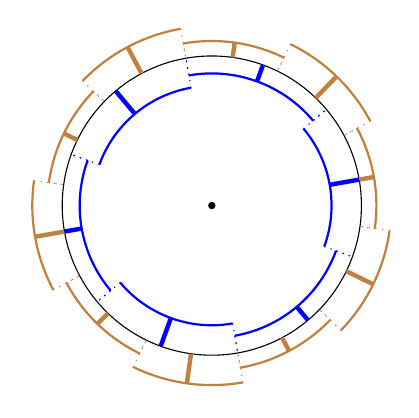
\begin{tikzpicture}[scale=1.9]
      \node (zero) at (0,0) {};
      \draw (zero) circle (1cm);

      %%%%%%%%%%%%%%%%%%%%%%%%%%%%%%%%%%%%%%%%%%%%%%%%%%%%%%%%%%%%%%%%%%%%%%%%%%%
      \foreach \w in {10}
      % {\foreach \sep in {0,45,90,135,180,225,270,315}
      {\foreach \sep in {0,36,72,108,144,180,216,252,288,324}
       {%\draw[thick,purple] (0,0) -- +({cos( \w + \sep )},{sin( \w + \sep )});

        \pgfmathsetmacro\r{{1.1 + mod(\w,10)/100 + mod(\sep,72)/360}}
        \draw[ultra thick,brown] ({cos( \w + \sep )},{sin( \w + \sep )})
          -- ({cos( \w + \sep) * \r},{sin( \w + \sep) * \r});

        \draw[thick,brown] ({cos( \w + \sep -18) * \r},{sin( \w + \sep -18) * \r})
          arc ({\w + \sep - 18}:{\w + \sep +18}:\r);

        \draw[dotted,brown] ({cos( \w + \sep -18) * \r},{sin( \w + \sep -18) * \r})
          -- ({cos( \w + \sep -18) * 1},{sin( \w + \sep -18) * 1});
        \draw[dotted,brown] ({cos( \w + \sep +18) * \r},{sin( \w + \sep +18) * \r})
          -- ({cos( \w + \sep +18) * 1},{sin( \w + \sep +18) * 1});
        }};

      %%%%%%%%%%%%%%%%%%%%%%%%%%%%%%%%%%%%%%%%%%%%%%%%%%%%%%%%%%%%%%%%%%%%%%%%%%%
      %%%%  Blue
      \foreach \w in {10}
      {\foreach \sep in {0,60,120,180,240,300}
       {%\draw[blue] (0,0) -- +({cos( \w + \sep ) * 0.9},{sin( \w + \sep ) * 0.9});

        \pgfmathsetmacro\r{{0.8 + mod(\w,10)/100 + mod(\sep,120)/720}}

        \draw[ultra thick,blue] ({cos( \w + \sep )},{sin( \w + \sep )})
          -- ({cos( \w + \sep) * \r},{sin( \w + \sep) * \r});
        \draw[thick,blue] ({cos( \w + \sep -30) * \r},{sin( \w + \sep -30) * \r})
          arc ({\w + \sep - 30}:{\w + \sep +30}:\r);


        \draw[dotted,blue] ({cos( \w + \sep -30) * \r},{sin( \w + \sep -30) * \r})
          -- ({cos( \w + \sep -30) * 1},{sin( \w + \sep -30) * 1});
        \draw[dotted,blue] ({cos( \w + \sep +30) * \r},{sin( \w + \sep +30) * \r})
          -- ({cos( \w + \sep +30) * 1},{sin( \w + \sep +30) * 1});
      }};


      % %%%%%%%%%%%%%%%%%%%%%%%%%%%%%%%%%%%%%%%%%%%%%%%%%%%%%%%%%%%%%%%%%%%%%%%%%%%
      % %%%%  Green
      % \foreach \w in {10}
      % {\foreach \sep in {0,90,180,270}
      %  {%\draw[green!60!black] (0,0) -- +({cos( \w + \sep ) * 0.8},{sin( \w + \sep) * 0.8});

      %   \pgfmathsetmacro\r{{0.8 + mod(\w,10)/100 + mod(\sep,180)/900}}

      %   \draw[ultra thick,green!60!black] ({cos( \w + \sep )},{sin( \w + \sep )})
      %     -- ({cos( \w + \sep) * \r},{sin( \w + \sep) * \r});
      %   \draw[thick,green!60!black] ({cos( \w + \sep -45) * \r},{sin( \w + \sep -45) * \r})
      %     arc ({\w + \sep - 45}:{\w + \sep +45}:\r);


      %   \draw[dotted,green!60!black] ({cos( \w + \sep -45) * \r},{sin( \w + \sep -45) * \r})
      %     -- ({cos( \w + \sep -45) * 1},{sin( \w + \sep -45) * 1});
      %   \draw[dotted,green!60!black] ({cos( \w + \sep +45) * \r},{sin( \w + \sep +45) * \r})
      %     -- ({cos( \w + \sep +45) * 1},{sin( \w + \sep +45) * 1});

      % }};

      \fill[white] (zero) circle (1.5pt);
      \fill (zero) circle (.7pt);
    \end{tikzpicture}
  \end{subfigure}%
  \begin{subfigure}[b]{0.33\textwidth}
    \caption{$\cK=\{\textcolor{purple}{5},\textcolor{green!60!black}{2}\}$}
    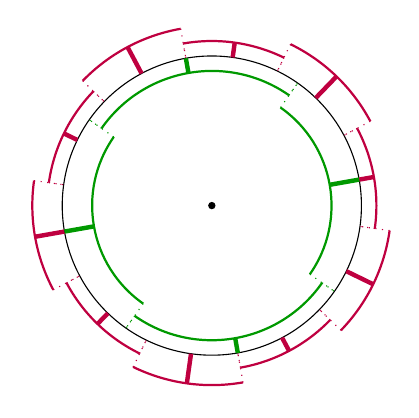
\begin{tikzpicture}[scale=1.9]
      \node (zero) at (0,0) {};
      \draw (zero) circle (1cm);

      %%%%%%%%%%%%%%%%%%%%%%%%%%%%%%%%%%%%%%%%%%%%%%%%%%%%%%%%%%%%%%%%%%%%%%%%%%%
      %%%%  Purple
      \foreach \w in {10}
      % {\foreach \sep in {0,45,90,135,180,225,270,315}
      {\foreach \sep in {0,36,72,108,144,180,216,252,288,324}
       {%\draw[thick,purple] (0,0) -- +({cos( \w + \sep )},{sin( \w + \sep )});

        \pgfmathsetmacro\r{{1.1 + mod(\w,10)/100 + mod(\sep,72)/360}}
        \draw[ultra thick,purple] ({cos( \w + \sep )},{sin( \w + \sep )})
          -- ({cos( \w + \sep) * \r},{sin( \w + \sep) * \r});

        \draw[thick,purple] ({cos( \w + \sep -18) * \r},{sin( \w + \sep -18) * \r})
          arc ({\w + \sep - 18}:{\w + \sep +18}:\r);

        \draw[dotted,purple] ({cos( \w + \sep -18) * \r},{sin( \w + \sep -18) * \r})
          -- ({cos( \w + \sep -18) * 1},{sin( \w + \sep -18) * 1});
        \draw[dotted,purple] ({cos( \w + \sep +18) * \r},{sin( \w + \sep +18) * \r})
          -- ({cos( \w + \sep +18) * 1},{sin( \w + \sep +18) * 1});
        }};

      % %%%%%%%%%%%%%%%%%%%%%%%%%%%%%%%%%%%%%%%%%%%%%%%%%%%%%%%%%%%%%%%%%%%%%%%%%%%
      % %%%%  Blue
      % \foreach \w in {10}
      % {\foreach \sep in {0,60,120,180,240,300}
      %  {%\draw[blue] (0,0) -- +({cos( \w + \sep ) * 0.9},{sin( \w + \sep ) * 0.9});

      %   \pgfmathsetmacro\r{{0.8 + mod(\w,10)/100 + mod(\sep,120)/720}}

      %   \draw[ultra thick,blue] ({cos( \w + \sep )},{sin( \w + \sep )})
      %     -- ({cos( \w + \sep) * \r},{sin( \w + \sep) * \r});
      %   \draw[thick,blue] ({cos( \w + \sep -30) * \r},{sin( \w + \sep -30) * \r})
      %     arc ({\w + \sep - 30}:{\w + \sep +30}:\r);


      %   \draw[dotted,blue] ({cos( \w + \sep -30) * \r},{sin( \w + \sep -30) * \r})
      %     -- ({cos( \w + \sep -30) * 1},{sin( \w + \sep -30) * 1});
      %   \draw[dotted,blue] ({cos( \w + \sep +30) * \r},{sin( \w + \sep +30) * \r})
      %     -- ({cos( \w + \sep +30) * 1},{sin( \w + \sep +30) * 1});
      % }};


      %%%%%%%%%%%%%%%%%%%%%%%%%%%%%%%%%%%%%%%%%%%%%%%%%%%%%%%%%%%%%%%%%%%%%%%%%%%
      %%%%  Green
      \foreach \w in {10}
      {\foreach \sep in {0,90,180,270}
       {%\draw[green!60!black] (0,0) -- +({cos( \w + \sep ) * 0.8},{sin( \w + \sep) * 0.8});

        \pgfmathsetmacro\r{{0.8 + mod(\w,10)/100 + mod(\sep,180)/900}}

        \draw[ultra thick,green!60!black] ({cos( \w + \sep )},{sin( \w + \sep )})
          -- ({cos( \w + \sep) * \r},{sin( \w + \sep) * \r});
        \draw[thick,green!60!black] ({cos( \w + \sep -45) * \r},{sin( \w + \sep -45) * \r})
          arc ({\w + \sep - 45}:{\w + \sep +45}:\r);


        \draw[dotted,green!60!black] ({cos( \w + \sep -45) * \r},{sin( \w + \sep -45) * \r})
          -- ({cos( \w + \sep -45) * 1},{sin( \w + \sep -45) * 1});
        \draw[dotted,green!60!black] ({cos( \w + \sep +45) * \r},{sin( \w + \sep +45) * \r})
          -- ({cos( \w + \sep +45) * 1},{sin( \w + \sep +45) * 1});

      }};

      \fill[white] (zero) circle (1.5pt);
      \fill (zero) circle (.7pt);
    \end{tikzpicture}
  \end{subfigure}%
  \begin{subfigure}[b]{0.33\textwidth}
    \caption{$\cK=\{\textcolor{blue}{3},\textcolor{green!60!black}{2}\}$}
    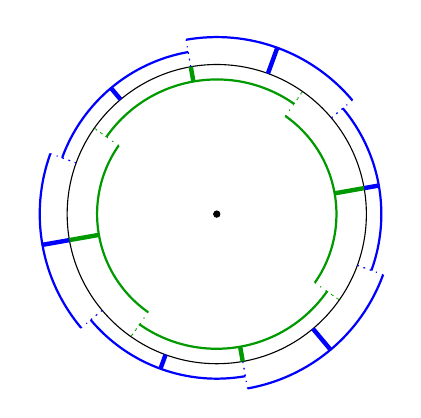
\begin{tikzpicture}[scale=1.9]
      \node (zero) at (0,0) {};
      \draw (zero) circle (1cm);

      %%%%%%%%%%%%%%%%%%%%%%%%%%%%%%%%%%%%%%%%%%%%%%%%%%%%%%%%%%%%%%%%%%%%%%%%%%%
      %%%%  Purple
      % \foreach \w in {10}
      % % {\foreach \sep in {0,45,90,135,180,225,270,315}
      % {\foreach \sep in {0,36,72,108,144,180,216,252,288,324}
      %  {%\draw[thick,purple] (0,0) -- +({cos( \w + \sep )},{sin( \w + \sep )});

      %   \pgfmathsetmacro\r{{1.1 + mod(\w,10)/100 + mod(\sep,72)/360}}
      %   \draw[ultra thick,purple] ({cos( \w + \sep )},{sin( \w + \sep )})
      %     -- ({cos( \w + \sep) * \r},{sin( \w + \sep) * \r});

      %   \draw[thick,purple] ({cos( \w + \sep -18) * \r},{sin( \w + \sep -18) * \r})
      %     arc ({\w + \sep - 18}:{\w + \sep +18}:\r);

      %   \draw[dotted,purple] ({cos( \w + \sep -18) * \r},{sin( \w + \sep -18) * \r})
      %     -- ({cos( \w + \sep -18) * 1},{sin( \w + \sep -18) * 1});
      %   \draw[dotted,purple] ({cos( \w + \sep +18) * \r},{sin( \w + \sep +18) * \r})
      %     -- ({cos( \w + \sep +18) * 1},{sin( \w + \sep +18) * 1});
      %   }};

      %%%%%%%%%%%%%%%%%%%%%%%%%%%%%%%%%%%%%%%%%%%%%%%%%%%%%%%%%%%%%%%%%%%%%%%%%%%
      %%%%  Blue
      \foreach \w in {10}
      {\foreach \sep in {0,60,120,180,240,300}
       {%\draw[blue] (0,0) -- +({cos( \w + \sep ) * 0.9},{sin( \w + \sep ) * 0.9});

        \pgfmathsetmacro\r{{1.1 + mod(\w,10)/100 + mod(\sep,120)/720}}

        \draw[ultra thick,blue] ({cos( \w + \sep )},{sin( \w + \sep )})
          -- ({cos( \w + \sep) * \r},{sin( \w + \sep) * \r});
        \draw[thick,blue] ({cos( \w + \sep -30) * \r},{sin( \w + \sep -30) * \r})
          arc ({\w + \sep - 30}:{\w + \sep +30}:\r);


        \draw[dotted,blue] ({cos( \w + \sep -30) * \r},{sin( \w + \sep -30) * \r})
          -- ({cos( \w + \sep -30) * 1},{sin( \w + \sep -30) * 1});
        \draw[dotted,blue] ({cos( \w + \sep +30) * \r},{sin( \w + \sep +30) * \r})
          -- ({cos( \w + \sep +30) * 1},{sin( \w + \sep +30) * 1});
      }};


      %%%%%%%%%%%%%%%%%%%%%%%%%%%%%%%%%%%%%%%%%%%%%%%%%%%%%%%%%%%%%%%%%%%%%%%%%%%
      %%%%  Green
      \foreach \w in {10}
      {\foreach \sep in {0,90,180,270}
       {%\draw[green!60!black] (0,0) -- +({cos( \w + \sep ) * 0.8},{sin( \w + \sep) * 0.8});

        \pgfmathsetmacro\r{{0.8 + mod(\w,10)/100 + mod(\sep,180)/900}}

        \draw[ultra thick,green!60!black] ({cos( \w + \sep )},{sin( \w + \sep )})
          -- ({cos( \w + \sep) * \r},{sin( \w + \sep) * \r});
        \draw[thick,green!60!black] ({cos( \w + \sep -45) * \r},{sin( \w + \sep -45) * \r})
          arc ({\w + \sep - 45}:{\w + \sep +45}:\r);


        \draw[dotted,green!60!black] ({cos( \w + \sep -45) * \r},{sin( \w + \sep -45) * \r})
          -- ({cos( \w + \sep -45) * 1},{sin( \w + \sep -45) * 1});
        \draw[dotted,green!60!black] ({cos( \w + \sep +45) * \r},{sin( \w + \sep +45) * \r})
          -- ({cos( \w + \sep +45) * 1},{sin( \w + \sep +45) * 1});

      }};

      \fill[white] (zero) circle (1.5pt);
      \fill (zero) circle (.7pt);
    \end{tikzpicture}
  \end{subfigure}
  \begin{subfigure}[b]{0.33\textwidth}
    \caption{$\cK=\{\textcolor{orange}{6},\textcolor{blue}{3}\}$}
    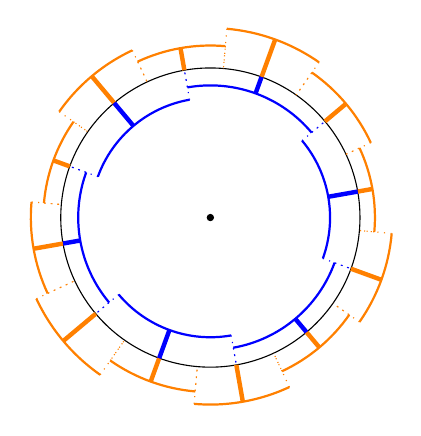
\begin{tikzpicture}[scale=1.9]
      \node (zero) at (0,0) {};
      \draw (zero) circle (1cm);

      %%%%%%%%%%%%%%%%%%%%%%%%%%%%%%%%%%%%%%%%%%%%%%%%%%%%%%%%%%%%%%%%%%%%%%%%%%%
      %%%%  Purple
      \foreach \w in {10}
      % {\foreach \sep in {0,45,90,135,180,225,270,315}
      {\foreach \sep in
        {0,30,60,90,120,150,180,210,240,270,300,330}
       {%\draw[thick,purple] (0,0) -- +({cos( \w + \sep )},{sin( \w + \sep )});

        \pgfmathsetmacro\hangle{15}

        \pgfmathsetmacro\r{{1.1 + mod(\w,10)/100 + mod(\sep,72)/360}}
        \draw[ultra thick,orange] ({cos( \w + \sep )},{sin( \w + \sep )})
          -- ({cos( \w + \sep) * \r},{sin( \w + \sep) * \r});

        \draw[thick,orange] ({cos( \w + \sep -\hangle) * \r},{sin( \w + \sep -\hangle) * \r})
          arc ({\w + \sep - \hangle}:{\w + \sep +\hangle}:\r);

        \draw[dotted,orange] ({cos( \w + \sep -\hangle) * \r},{sin( \w + \sep -\hangle) * \r})
          -- ({cos( \w + \sep -\hangle) * 1},{sin( \w + \sep -\hangle) * 1});
        \draw[dotted,orange] ({cos( \w + \sep +\hangle) * \r},{sin( \w + \sep +\hangle) * \r})
          -- ({cos( \w + \sep +\hangle) * 1},{sin( \w + \sep +\hangle) * 1});
        }};

      %%%%%%%%%%%%%%%%%%%%%%%%%%%%%%%%%%%%%%%%%%%%%%%%%%%%%%%%%%%%%%%%%%%%%%%%%%%
      \foreach \w in {10}
      {\foreach \sep in {0,60,120,180,240,300}
       {%\draw[blue] (0,0) -- +({cos( \w + \sep ) * 0.9},{sin( \w + \sep ) * 0.9});

        \pgfmathsetmacro\r{{0.8 + mod(\w,10)/100 + mod(\sep,120)/720}}

        \draw[ultra thick,blue] ({cos( \w + \sep )},{sin( \w + \sep )})
          -- ({cos( \w + \sep) * \r},{sin( \w + \sep) * \r});
        \draw[thick,blue] ({cos( \w + \sep -30) * \r},{sin( \w + \sep -30) * \r})
          arc ({\w + \sep - 30}:{\w + \sep +30}:\r);


        \draw[dotted,blue] ({cos( \w + \sep -30) * \r},{sin( \w + \sep -30) * \r})
          -- ({cos( \w + \sep -30) * 1},{sin( \w + \sep -30) * 1});
        \draw[dotted,blue] ({cos( \w + \sep +30) * \r},{sin( \w + \sep +30) * \r})
          -- ({cos( \w + \sep +30) * 1},{sin( \w + \sep +30) * 1});
      }};

      \fill[white] (zero) circle (1.5pt);
      \fill (zero) circle (.7pt);
    \end{tikzpicture}
  \end{subfigure}
  \begin{subfigure}[b]{0.33\textwidth}
    \caption{$\cK=\{\textcolor{purple}{7},\textcolor{blue}{3}\}$}
    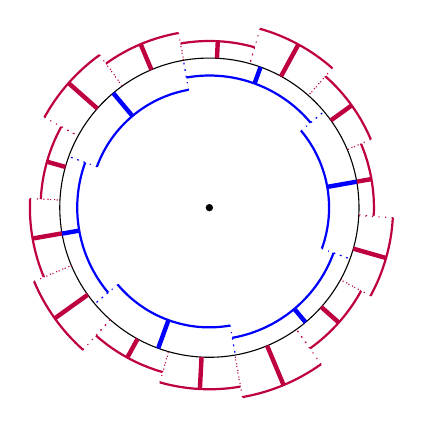
\begin{tikzpicture}[scale=1.9]
      \node (zero) at (0,0) {};
      \draw (zero) circle (1cm);

      %%%%%%%%%%%%%%%%%%%%%%%%%%%%%%%%%%%%%%%%%%%%%%%%%%%%%%%%%%%%%%%%%%%%%%%%%%%
      %%%%  Purple
      \foreach \w in {10}
      % {\foreach \sep in {0,45,90,135,180,225,270,315}
      {\foreach \sep in
        {0,25.7,51.4,77.1,102.8,128.5,154.2,179.9,205.6,231.3,257.0,282.7,308.4,334.1}
       {%\draw[thick,purple] (0,0) -- +({cos( \w + \sep )},{sin( \w + \sep )});

        \pgfmathsetmacro\r{{1.1 + mod(\w,10)/100 + mod(\sep,72)/360}}
        \draw[ultra thick,purple] ({cos( \w + \sep )},{sin( \w + \sep )})
          -- ({cos( \w + \sep) * \r},{sin( \w + \sep) * \r});

        \draw[thick,purple] ({cos( \w + \sep -12.8) * \r},{sin( \w + \sep -12.8) * \r})
          arc ({\w + \sep - 12.8}:{\w + \sep +12.8}:\r);

        \draw[dotted,purple] ({cos( \w + \sep -12.8) * \r},{sin( \w + \sep -12.8) * \r})
          -- ({cos( \w + \sep -12.8) * 1},{sin( \w + \sep -12.8) * 1});
        \draw[dotted,purple] ({cos( \w + \sep +12.8) * \r},{sin( \w + \sep +12.8) * \r})
          -- ({cos( \w + \sep +12.8) * 1},{sin( \w + \sep +12.8) * 1});
        }};

      %%%%%%%%%%%%%%%%%%%%%%%%%%%%%%%%%%%%%%%%%%%%%%%%%%%%%%%%%%%%%%%%%%%%%%%%%%%
      \foreach \w in {10}
      {\foreach \sep in {0,60,120,180,240,300}
       {%\draw[blue] (0,0) -- +({cos( \w + \sep ) * 0.9},{sin( \w + \sep ) * 0.9});

        \pgfmathsetmacro\r{{0.8 + mod(\w,10)/100 + mod(\sep,120)/720}}

        \draw[ultra thick,blue] ({cos( \w + \sep )},{sin( \w + \sep )})
          -- ({cos( \w + \sep) * \r},{sin( \w + \sep) * \r});
        \draw[thick,blue] ({cos( \w + \sep -30) * \r},{sin( \w + \sep -30) * \r})
          arc ({\w + \sep - 30}:{\w + \sep +30}:\r);


        \draw[dotted,blue] ({cos( \w + \sep -30) * \r},{sin( \w + \sep -30) * \r})
          -- ({cos( \w + \sep -30) * 1},{sin( \w + \sep -30) * 1});
        \draw[dotted,blue] ({cos( \w + \sep +30) * \r},{sin( \w + \sep +30) * \r})
          -- ({cos( \w + \sep +30) * 1},{sin( \w + \sep +30) * 1});
      }};

      \fill[white] (zero) circle (1.5pt);
      \fill (zero) circle (.7pt);
    \end{tikzpicture}
  \end{subfigure}
  \begin{subfigure}[b]{0.33\textwidth}
    \caption{$\cK=\{\textcolor{orange}{6},\textcolor{green!60!black}{2}\}$}
    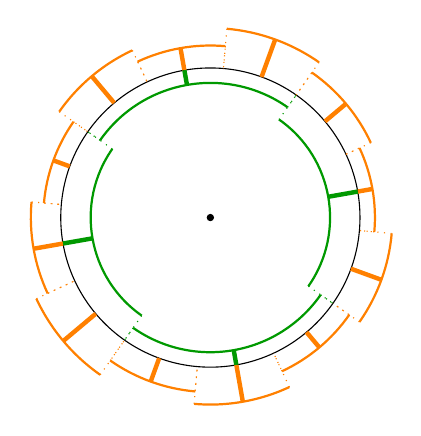
\begin{tikzpicture}[scale=1.9]
      \node (zero) at (0,0) {};
      \draw (zero) circle (1cm);

      %%%%%%%%%%%%%%%%%%%%%%%%%%%%%%%%%%%%%%%%%%%%%%%%%%%%%%%%%%%%%%%%%%%%%%%%%%%
      %%%%  Purple
      \foreach \w in {10}
      % {\foreach \sep in {0,45,90,135,180,225,270,315}
      {\foreach \sep in
        {0,30,60,90,120,150,180,210,240,270,300,330}
       {%\draw[thick,purple] (0,0) -- +({cos( \w + \sep )},{sin( \w + \sep )});

        \pgfmathsetmacro\hangle{15}

        \pgfmathsetmacro\r{{1.1 + mod(\w,10)/100 + mod(\sep,72)/360}}
        \draw[ultra thick,orange] ({cos( \w + \sep )},{sin( \w + \sep )})
          -- ({cos( \w + \sep) * \r},{sin( \w + \sep) * \r});

        \draw[thick,orange] ({cos( \w + \sep -\hangle) * \r},{sin( \w + \sep -\hangle) * \r})
          arc ({\w + \sep - \hangle}:{\w + \sep +\hangle}:\r);

        \draw[dotted,orange] ({cos( \w + \sep -\hangle) * \r},{sin( \w + \sep -\hangle) * \r})
          -- ({cos( \w + \sep -\hangle) * 1},{sin( \w + \sep -\hangle) * 1});
        \draw[dotted,orange] ({cos( \w + \sep +\hangle) * \r},{sin( \w + \sep +\hangle) * \r})
          -- ({cos( \w + \sep +\hangle) * 1},{sin( \w + \sep +\hangle) * 1});
        }};

      %%%%%%%%%%%%%%%%%%%%%%%%%%%%%%%%%%%%%%%%%%%%%%%%%%%%%%%%%%%%%%%%%%%%%%%%%%%
      %%%%  Green
      \foreach \w in {10}
      {\foreach \sep in {0,90,180,270}
       {%\draw[green!60!black] (0,0) -- +({cos( \w + \sep ) * 0.8},{sin( \w + \sep) * 0.8});

        \pgfmathsetmacro\r{{0.8 + mod(\w,10)/100 + mod(\sep,180)/900}}

        \draw[ultra thick,green!60!black] ({cos( \w + \sep )},{sin( \w + \sep )})
          -- ({cos( \w + \sep) * \r},{sin( \w + \sep) * \r});
        \draw[thick,green!60!black] ({cos( \w + \sep -45) * \r},{sin( \w + \sep -45) * \r})
          arc ({\w + \sep - 45}:{\w + \sep +45}:\r);


        \draw[dotted,green!60!black] ({cos( \w + \sep -45) * \r},{sin( \w + \sep -45) * \r})
          -- ({cos( \w + \sep -45) * 1},{sin( \w + \sep -45) * 1});
        \draw[dotted,green!60!black] ({cos( \w + \sep +45) * \r},{sin( \w + \sep +45) * \r})
          -- ({cos( \w + \sep +45) * 1},{sin( \w + \sep +45) * 1});

      }};

      \fill[white] (zero) circle (1.5pt);
      \fill (zero) circle (.7pt);
    \end{tikzpicture}
  \end{subfigure}
  \begin{subfigure}[b]{0.33\textwidth}
    \caption{$\cK=\{\textcolor{purple}{7},\textcolor{green!60!black}{2}\}$}
    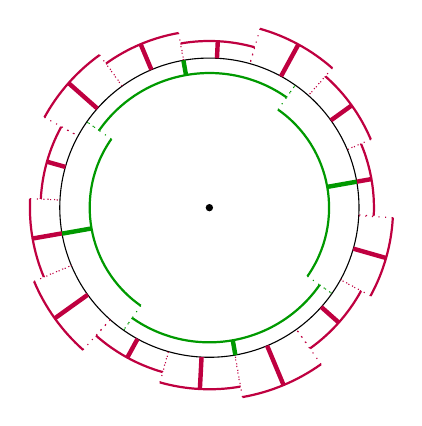
\begin{tikzpicture}[scale=1.9]
      \node (zero) at (0,0) {};
      \draw (zero) circle (1cm);

      %%%%%%%%%%%%%%%%%%%%%%%%%%%%%%%%%%%%%%%%%%%%%%%%%%%%%%%%%%%%%%%%%%%%%%%%%%%
      %%%%  Purple
      \foreach \w in {10}
      % {\foreach \sep in {0,45,90,135,180,225,270,315}
      {\foreach \sep in
        {0,25.7,51.4,77.1,102.8,128.5,154.2,179.9,205.6,231.3,257.0,282.7,308.4,334.1}
       {%\draw[thick,purple] (0,0) -- +({cos( \w + \sep )},{sin( \w + \sep )});

        \pgfmathsetmacro\r{{1.1 + mod(\w,10)/100 + mod(\sep,72)/360}}
        \draw[ultra thick,purple] ({cos( \w + \sep )},{sin( \w + \sep )})
          -- ({cos( \w + \sep) * \r},{sin( \w + \sep) * \r});

        \draw[thick,purple] ({cos( \w + \sep -12.8) * \r},{sin( \w + \sep -12.8) * \r})
          arc ({\w + \sep - 12.8}:{\w + \sep +12.8}:\r);

        \draw[dotted,purple] ({cos( \w + \sep -12.8) * \r},{sin( \w + \sep -12.8) * \r})
          -- ({cos( \w + \sep -12.8) * 1},{sin( \w + \sep -12.8) * 1});
        \draw[dotted,purple] ({cos( \w + \sep +12.8) * \r},{sin( \w + \sep +12.8) * \r})
          -- ({cos( \w + \sep +12.8) * 1},{sin( \w + \sep +12.8) * 1});
        }};

      %%%%%%%%%%%%%%%%%%%%%%%%%%%%%%%%%%%%%%%%%%%%%%%%%%%%%%%%%%%%%%%%%%%%%%%%%%%
      %%%%  Green
      \foreach \w in {10}
      {\foreach \sep in {0,90,180,270}
       {%\draw[green!60!black] (0,0) -- +({cos( \w + \sep ) * 0.8},{sin( \w + \sep) * 0.8});

        \pgfmathsetmacro\r{{0.8 + mod(\w,10)/100 + mod(\sep,180)/900}}

        \draw[ultra thick,green!60!black] ({cos( \w + \sep )},{sin( \w + \sep )})
          -- ({cos( \w + \sep) * \r},{sin( \w + \sep) * \r});
        \draw[thick,green!60!black] ({cos( \w + \sep -45) * \r},{sin( \w + \sep -45) * \r})
          arc ({\w + \sep - 45}:{\w + \sep +45}:\r);


        \draw[dotted,green!60!black] ({cos( \w + \sep -45) * \r},{sin( \w + \sep -45) * \r})
          -- ({cos( \w + \sep -45) * 1},{sin( \w + \sep -45) * 1});
        \draw[dotted,green!60!black] ({cos( \w + \sep +45) * \r},{sin( \w + \sep +45) * \r})
          -- ({cos( \w + \sep +45) * 1},{sin( \w + \sep +45) * 1});

      }};

      \fill[white] (zero) circle (1.5pt);
      \fill (zero) circle (.7pt);
    \end{tikzpicture}
  \end{subfigure}
  \caption{Ideas for examples with two levels.}
\end{figure} %}}}

%%%%%%%%%%%%%%%%%%%%%%%%%%%%%%%%%%%%%%%%%%%%%%%%%%%%%%%%%%%%%%%%%%%%%%%%%%%%%%%
\section{Building our example}
We want to have a unramified connection with more than one level. Two levels
might be enough. Our plan is as follows:
\begin{enumerate}
  \item fix some determining polynomials, which define the levels and
    anti-Stokes directions;
  \item fix some exponent of formal monodromy $L$, which defines, together with
    the determining polynomials and the order, our normal form $A^0$;
  \item fix some formal transformation $\hat F$, which defines our system
    $A:={}^{\hat F}\!A^0$.
\end{enumerate}

\paragraph{Fix the determining polynomials}
Let us start by defining the determining polynomials $q_j(t^{-1})$ of levels
$l_j$.
Thus we have
\begin{itemize}
  \item the leading factor $a_{jl}\in\C\backslash\{0\}$,
  \item the leading coefficient $\frac{a_{jl}}{t^{k}}=q_{jl}(t^{-1})$ and
  \item the degree $k_{jl}$
\end{itemize}
of $q_j-q_l\in\cQ_{[\End A^0]}$
(cf.\ definition~\ref{defn:determiningPolysOfEndA})
from which we deduce the anti-Stokes directions
$\A=\{\theta_1,\dots,\theta_\nu\}$.

\rewrite{We want to create an example} with levels $\cK=\{k_1<k_2\}$ thus we
need at least three different determining polynomials.
If we assume that all determining polynomials have different leading terms, we
require (Up to permutation) that the first $n'$, $0<n'<n$,
polynomials should have degree $l_j=k_2$.
For $n'<j<n$ the polynomials $q_j$ should have degree $l_j\leq k_1$ and the
last polynomial $q_n$ is allowed to be of degree $l_n\leq k_1$.
We will choose $l_1=7$, $l_2=2$ and $l_3=0$.
\begin{comment}
  Thus
  \begin{align*}
    q_1= \frac{a_1^7}{t^7}+ \sum_{j\in\{1,\dots,6\}}\frac{a_1^j}{t^j}
  &&\text{,}&&q_2= \frac{a_2^2}{t^2}+ \frac{a_2^1}{t^1}
  &&\text{and}&&q_3=0
  \end{align*}
  and the differences are given by
  \begin{align*}
    q_1-q_2= \frac{a_1^7}{t^7}+
      \cdots+
      \frac{a_1^3}{t^3}+ \frac{a_1^2-a_2^2}{t^2}+
      \frac{a_1^1-a_2^1}{t^1}
  &&\text{,}&&q_1-q_3=q_1
  &&\text{and}&&q_2-q_3=q_2
  \end{align*}
\end{comment}

\paragraph{Fix the exponent of formal monodromy}
We then construct the connection matrix by
% \begin{paracol}{2}\sloppy
% \switchcolumn[0]\noindent
  \[
    A^0=Q'(t^{-1})+L\frac{1}{t} \in G(\!\{t\}\!)
  \]
% \switchcolumn[1]\noindent
%   \[
%     \textcolor{red}{\text{or~}A^0=dQ(t^{-1})+L\frac{dt}{d}}
%   \]
% \end{paracol}
where
\begin{itemize}
  \item $Q(t^{-1})=\diag(q_1(t^{-1}),q_2(t^{-1}),\dots,q_n(t^{-1}))$
    and
  \item $L$ is constant diagonal and invertible.
\end{itemize}

\begin{lem}
  \marginnote{\cite[4f]{thboalch}}
  \TODO[move to fund-sol-defn]
  The matrix $\cY_0:=t^Le^{Q(t^{-1})}$ is then a fundamental solution of
  $[A^0]$.
\end{lem}
\begin{proof}
  It is sufficient to show that $\cY\in G(\!\{t\}\!)$, i.e.\ is invertible, and
  that its columns are solutions.

  Since we are dealing with diagonal matrices it is easy to see, that
  \begin{align*}
    \frac{d}{dt}e^{Q(t^{-1})}
    &=\diag\left(\frac{d}{dt}e^{q_1(t^{-1})},\frac{d}{dt}e^{q_2(t^{-1})},\dots,
      \frac{d}{dt}e^{q_n(t^{-1})}\right)
      \\&=\diag\left(\frac{d}{dt}q_1(t^{-1})e^{q_1(t^{-1})}
                    ,\frac{d}{dt}q_1(t^{-1})e^{q_2(t^{-1})}
                    ,\dots
                    ,\frac{d}{dt}q_1(t^{-1})e^{q_n(t^{-1})}\right)
  \\&=Q'(t^{-1})e^{Q(t^{-1})} \,.
  \end{align*}
  and, since the function $t^L$ is defined as $e^{L\ln t}$,
  \begin{align*}
    \frac{d}{dt}t^L&=\frac{d}{dt}e^{L\ln t}
  \\&=Le^{(L-\id)\ln t}
  \\&=L\frac{1}{t}t^L \,.
  \end{align*}
  Thus we can prove, that $\cY_0$ is a matrix consisting of solutions:
  \begin{align*}
    \frac{d}{dt}\cY_0
    &=\frac{d}{dt}\left(t^Le^{Q(t^{-1})}\right)
  \\&=\frac{d}{dt}t^Le^{Q(t^{-1})}+t^L\frac{d}{dt}e^{Q(t^{-1})}
  \\&=L\frac{1}{t}t^Le^{Q(t^{-1})}+t^LQ'(t^{-1})e^{Q(t^{-1})}
  \\&=L\frac{1}{t}t^Le^{Q(t^{-1})}+Q'(t^{-1})t^Le^{Q(t^{-1})}
  \\&=\left(Q'(t^{-1})+L\frac{1}{t}\right)t^Le^{Q(t^{-1})}
  \\&=A^0\cY_0
  \end{align*}
  The inevitability condition is clear.
\end{proof}

\paragraph{Fix the formal transformation}
Choose a formal transformation $\hat F\in\hat G(A^0)$, i.e.\ an ambassador of
an class in $G\backslash\hat G(A^0)$, and thus a connection matrix
${}^{\hat F}\!A^0$ and the corresponding fundamental solution
$\cY=\hat F\cY_0$.

From the theorem~\ref{thm:summaFaktori} we know in our case, that $\hat F$ can
be factored in
\[
  \hat F=\hat F_2 \hat F_1
\]
where $\hat F_j$ is
\begin{itemize}
  \item $k_j$-summable and
  \item with singular directions belonging to $\A^{k_j}$.
\end{itemize}
\TODO[build this way?]

\section{Find corresponding element in $\prod_{\theta\in\A}\Sto_\theta(A^0)$}
\begin{comment}
  needs \textbf{summability}?
  \begin{itemize}
    \item \cite[9]{thboalch} (only mentions multisummability)
    \item \cite[III.2]{Loday1994}
    \item \cite{Loday2014}
  \end{itemize}
\end{comment}

We then get
\[
  (\kappa_{\theta_1},\dots,\kappa_{\theta_\nu})
  \in\prod_{\theta\in\A}\Sto_\theta(A^0)
\]
by setting $\kappa_\theta:=
S^-_\theta(\hat F)\left(S^+_\theta(\hat F)\right)̂^{̀-1}\in\Sto_\theta(A^0)$
(cf.\ definition~\ref{defn:sumsLeftRight}).
\begin{rem}
  \TODO[Move to sec:Multisummability?]
  For each $\theta\in\A$ is $\kappa_\theta$
  \begin{enumerate}
    \item flat, since
      \begin{align*}
        \hat\kappa_\theta
        &=\hat{\left(F_\theta^+\right)̂^{̀-1}}\hat{F_\theta^-}
      \\&=\hat{F}^{̀-1}\hat{F}
      \\&=\id
      \end{align*}
    \item an isotropy, since
      \begin{align*}
        {}^{\kappa_\theta}\!A^0
        &= {}^{\left(F_\theta^+\right)̂^{̀-1}F_\theta^-}\!A^0
      \\&= {}^{\left(F_\theta^+\right)̂^{̀-1}}\!\left({}^{F_\theta^-}\!A^0\right)
      \\&\overset{\TODO{}}{=}{}^{\left(F_\theta^+\right)̂^{̀-1}}\!A^1
      \\&\overset{\TODO{}}{=}A^0
      \end{align*}
      \begin{comment}
        \begin{align*}
          {}^{\kappa_\theta}\!A^0
          &= (d\kappa_\theta)\kappa_\theta^{-1}+\kappa_\theta A^0
          \kappa_\theta^{-1}
        \\&=\left(
            d\left(\left(F_\theta^+\right)̂^{̀-1}\right)̂F_\theta^-
            +\left(F_\theta^+\right)̂^{̀-1}dF_\theta^-
          \right)\kappa_\theta^{-1}+\kappa_\theta A^0\kappa_\theta^{-1}
        \\&=\left(
            d\left(\left(F_\theta^+\right)̂^{̀-1}\right)̂F_\theta^-
            +\left(F_\theta^+\right)̂^{̀-1}dF_\theta^-
          \right) \left(F_\theta^-\right)̂^{̀-1}F_\theta^+
          +\left(F_\theta^+\right)̂^{̀-1}F_\theta^- A^0
           \left(F_\theta^-\right)̂^{̀-1}F_\theta^+
        \\&=
           d\left(\left(F_\theta^+\right)̂^{̀-1}\right)̂F_\theta^+
           +\left(F_\theta^+\right)̂^{̀-1}dF_\theta^-
           \left(F_\theta^-\right)̂^{̀-1}F_\theta^+
           +\left(F_\theta^+\right)̂^{̀-1}F_\theta^- A^0
           \left(F_\theta^-\right)̂^{̀-1}F_\theta^+
        \\&=\TODO{}
        \\&=A^0
        \end{align*}
      \end{comment}
    \item of maximal decay, since \TODO{}
  \end{enumerate}
\end{rem}

\subsection{How do the matrices $\kappa_\theta$ look like?}

\section{The corresponding element in $\St(A^0)$}
The map $h$ from theorem~\ref{thm:mainThm2} maps the element
$(\kappa_{\theta_1},\dots,\kappa_{\theta_\nu})$ to an element of $\St(A^0)$.
